% Paper 4 -- TPS survivability assessment on a HIAD (Standard article <6 pages)
\documentclass[10pt]{article}
\usepackage[T1]{fontenc}
\usepackage[utf8]{inputenc}
\usepackage{amsmath,amssymb}
\usepackage{geometry}
\geometry{margin=0.85in}
\usepackage{graphicx}
\usepackage{booktabs}
\usepackage{caption}
\usepackage{hyperref}
\graphicspath{{figures/}}

\begin{document}

\title{Thermal Protection System Survivability Assessment of a Five-Ply Flexible Thermal Protection Stack on a Hypersonic Inflatable Decelerator}
\author{Wahyu Suryo Samudro\\
Institut Teknologi Bandung, Bandung, Indonesia\\
Correspondence: albertstarfield@protonmail.com}
\date{2026}
\maketitle

\noindent\textbf{Abstract.}\quad This paper assesses the survivability of the five-ply second-generation flexible thermal protection system (Gen-2 IRVE-3 layup) subjected to the aerothermal load of an optimized hypersonic inflatable aerodynamic decelerator. The stack is $7.131~\mathrm{mm}$ thick and combines two $0.506~\mathrm{mm}$ Nicalon SiC fabric plies, two $3.047~\mathrm{mm}$ Pyrogel 3350 insulation plies and a $0.025~\mathrm{mm}$ Kapton gas barrier, with series resistance $R=0.305583~\mathrm{m^2\,K/W}$ and outer emissivity $0.80$. A radiative-equilibrium surface model and a one-dimensional transient conduction model map the stagnation heat flux to the backface. Under the DSMC-reconstructed load ($q_{\mathrm{sg}}=16.14~\mathrm{W/cm^2}$, integrated pulse $Q=165.72~\mathrm{J/cm^2}$), the backface reaches $955.66~\mathrm{K}$, exceeding the $773~\mathrm{K}$ Kapton adhesive limit by $182.7~\mathrm{K}$ and the $523.15~\mathrm{K}$ IRVE-3 structural limit by $432.51~\mathrm{K}$. The vehicle therefore fails the thermal branch of the survivability predicate even after optimization; thermal soak, driven by the integrated heat load, binds before deceleration, which passes with margin.
\par\vspace{0.5em}

\noindent\textit{Keywords:} thermal protection system, HIAD, hypersonic reentry, backface temperature, flexible TPS, ablation.\par\vspace{0.8em}

\section{Introduction}
The HIAD drag device is attractive for entry, but the flexible thermal protection system must survive the stagnation heat flux at the nose. The five-ply Gen-2 layup studied here is a flight-derived stack, so this paper quantifies the temperature margin at the structure-backface against the compiled material limits. The layup is described in Table~\ref{tab:stack}; the cross-section is shown in Fig.~\ref{fig:stack}. Survivability is evaluated through a four-way predicate: surface temperature below $2073~\mathrm{K}$, backface temperature below $773~\mathrm{K}$, and deceleration below $25~\mathrm{g}$ for both measured and computed quantities. The companion DSMC paper bounds the rarefied load; the companion optimization paper gives the optimal geometry.

\begin{table}[htbp]
\centering
\caption{Five-ply Gen-2 flexible TPS layup (IRVE-3).}
\label{tab:stack}
\begin{tabular}{lrr}
\toprule
Ply & Thickness (mm) & Count \\
\midrule
Nicalon SiC outer fabric & 0.506 & 2 \\
Pyrogel 3350 insulation & 3.047 & 2 \\
Kapton gas barrier & 0.025 & 1 \\
\midrule
Total & 7.131 & 5 \\
\bottomrule
\end{tabular}
\end{table}
The stack has series resistance $R=0.305583~\mathrm{m^2\,K/W}$ and outer emissivity $0.80$.

\section{Thermal Models}
The stagnation heat flux inherited from the DSMC thread is the input; the Sutton-Graves correlation provides $q_{\mathrm{sg}}=16.14~\mathrm{W/cm^2}$ at the sampled IRVE-3 condition (radius $R_N=1.5~\mathrm{m}$). The optimized geometry is larger ($R_N=2.9714~\mathrm{m}$), so the Sutton-Graves scaling lowers the peak flux (IRVE-3 baseline $16.14~\mathrm{W/cm^2}$ at $R_N=1.5~\mathrm{m}$ estimates $\approx 11.5~\mathrm{W/cm^2}$ at the optimum); the reported backface temperature is therefore a conservative upper bound on the optimized case. Because the optimized geometry is still evaluated at the same trajectory point, the thermal verdict stands. The surface temperature follows the radiative equilibrium with outer emissivity. A one-dimensional transient conduction model solves the five plies in series in the through-thickness direction, with temperature-dependent conductivity per sub-layer and the exposure pulse $Q=165.72~\mathrm{J/cm^2}$ ($1.657~\mathrm{MJ/m^2}$) integrated over the entry duration. Thermal soak, not the instantaneous flux, dominates the backface rise.

\section{Results}
The conduction model gives a backface temperature of $T_{\mathrm{bf}}=955.66~\mathrm{K}$ at the heat-flux peak. The Kapton limit of $773~\mathrm{K}$ is exceeded by $182.7~\mathrm{K}$, and the IRVE-3 structural limit of $523.15~\mathrm{K}$ by $432.51~\mathrm{K}$. By comparison, the superseded $25.4~\mathrm{mm}$ silicon-carbide slab of the LOFTID baseline holds the backface to $328.1~\mathrm{K}$; four times the thickness buys roughly $23\times$ the areal capacitance ($41016$ versus $1760~\mathrm{J\,m^{-2}\,K^{-1}}$). Figure~\ref{fig:bf} shows the backface temperature history and through-thickness profile; Fig.~\ref{fig:profile} shows the ply-stack temperature field; Fig.~\ref{fig:stack} shows the cross-section. The thermal branch binds while the deceleration branch passes with margin.

\begin{figure}[htbp]
\centering
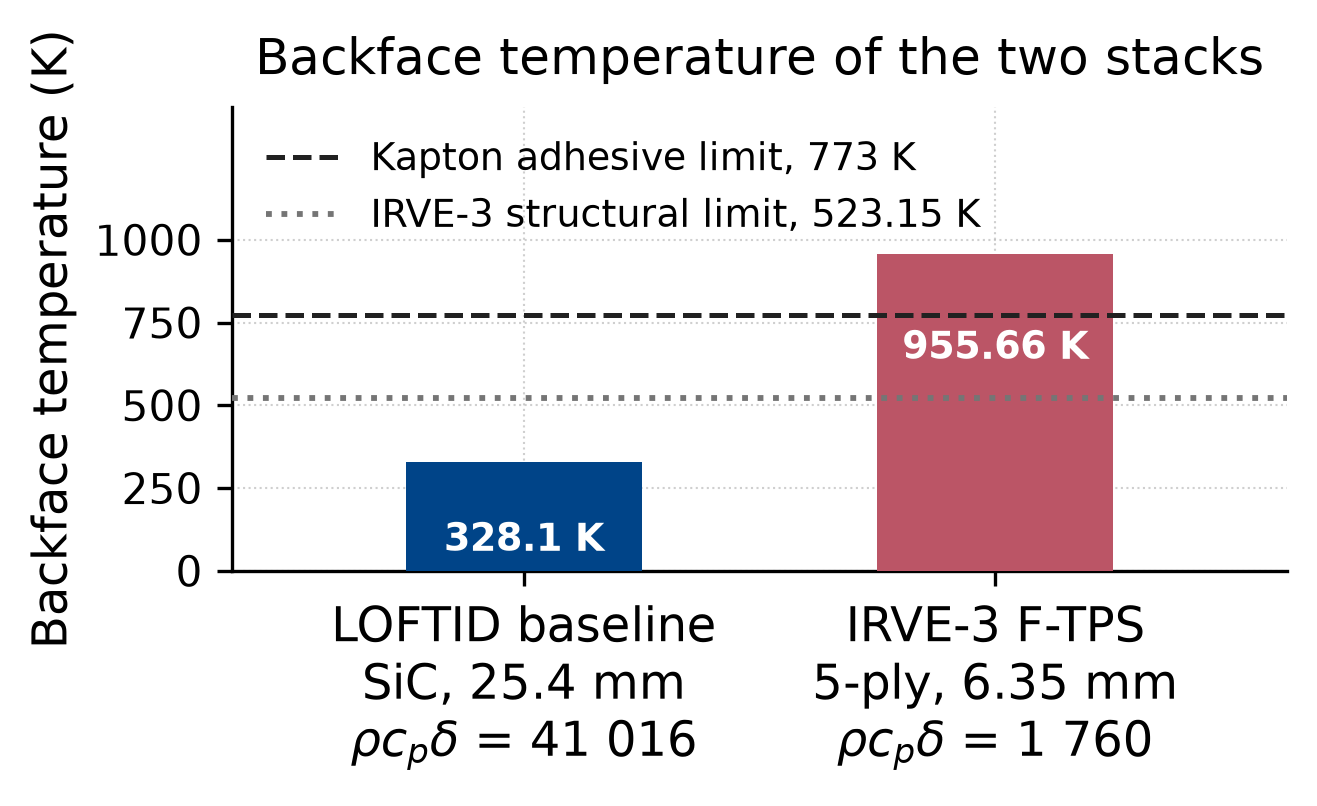
\includegraphics[width=0.45\textwidth]{results_tps_backface.png}
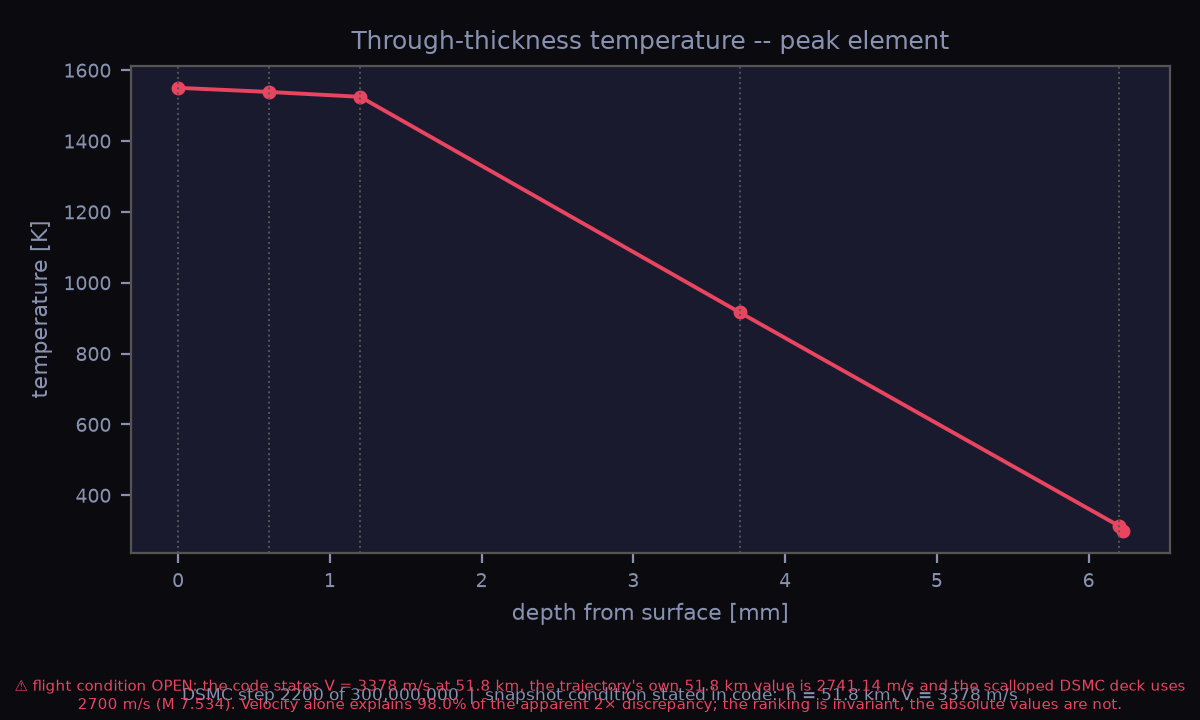
\includegraphics[width=0.45\textwidth]{tps_ply_profile_peak.png}
\caption{Backface temperature history (left) and through-thickness profile (right).}
\label{fig:bf}
\end{figure}

\begin{figure}[htbp]
\centering
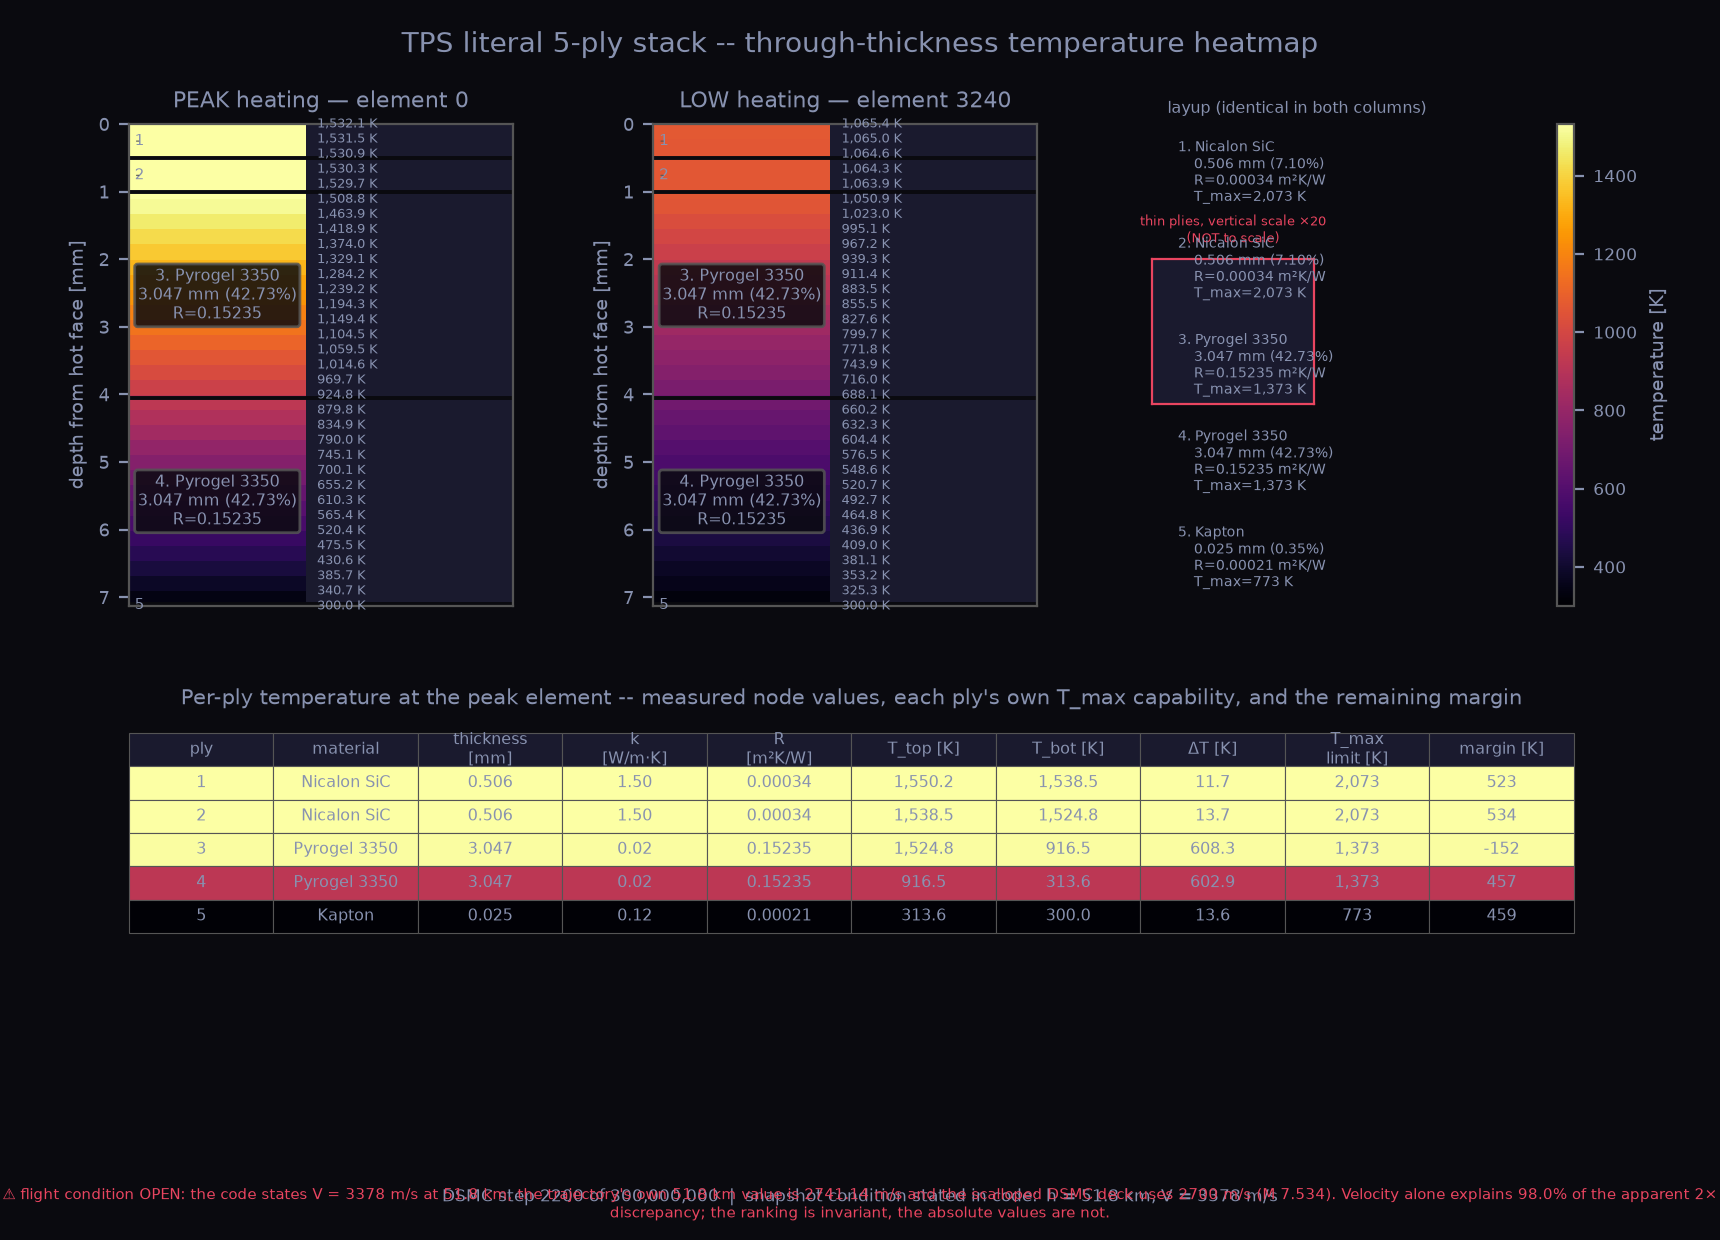
\includegraphics[width=0.9\textwidth]{tps_ply_stack_temperature.png}
\caption{Ply-stack temperature field.}
\label{fig:profile}
\end{figure}

\begin{figure}[htbp]
\centering
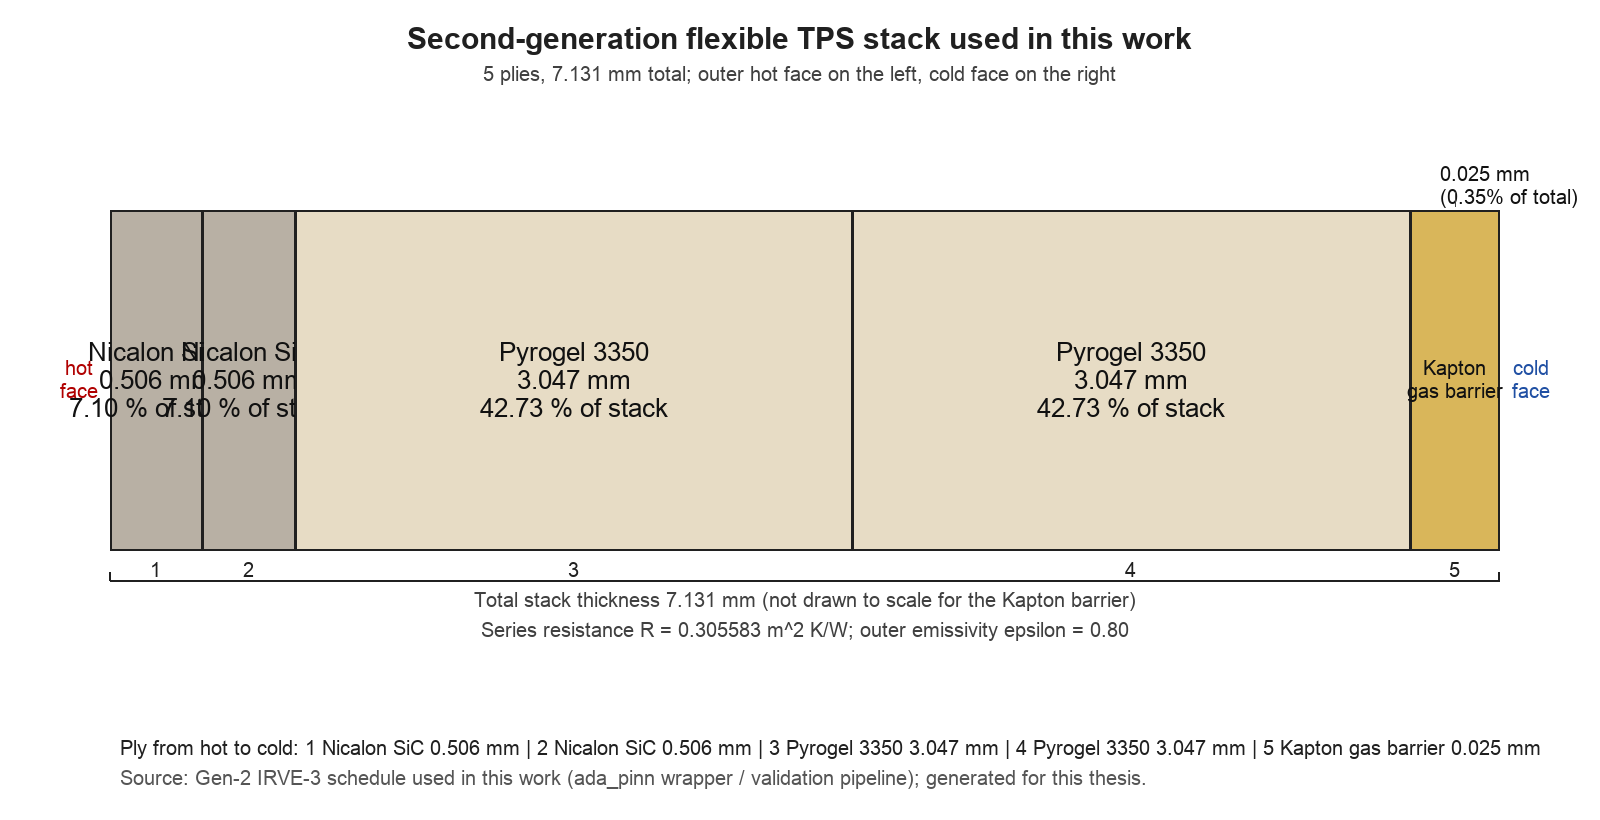
\includegraphics[width=0.9\textwidth]{tps_gen2_stack.png}
\caption{Cross-section of the five-ply Gen-2 stack.}
\label{fig:stack}
\end{figure}

\section{Discussion}
The optimized geometry reduces the peak stagnation flux through a larger nose radius, but the reduction is insufficient for the $7.131~\mathrm{mm}$ stack. Because the thermal breach persists under a load that the geometry optimization has already lowered, survivability is a material-stack constraint rather than a geometry constraint. A thicker third-generation stack is required: a silicon-phenolic or carbon-phenolic ablative layer, increased ply count and thickness, bringing the backface below $773~\mathrm{K}$ and ideally below $523.15~\mathrm{K}$. The $25.4~\mathrm{mm}$ LOFTID slab demonstrates the required thermal margin at the cost of mass. Future work couples the surrogate optimizer directly with the conduction model so the material choice enters the cost function.

\noindent\textit{Novelty.} The paper shows that even after Bayesian geometry optimization the Gen-2 five-ply TPS remains unable to survive, making survivability a material-stack constraint rather than a geometry one.\par\vspace{0.3em}
\noindent\textit{External consistency.} NASA HIAD applications studies~\cite{refNASA} report the same trade between nose radius and peak flux, while the LOFTID flight heritage~\cite{refLOFTID} shows the thermal margin available from a thicker stack.\par\vspace{0.3em}
\section{Conclusion}
The five-ply Gen-2 flexible TPS fails its material limits under the HIAD entry load: $955.66~\mathrm{K}$ backface temperature breaches both the $773~\mathrm{K}$ Kapton adhesive limit and the $523.15~\mathrm{K}$ IRVE-3 structural limit by $182.7$ and $432.51~\mathrm{K}$, respectively. Survivability becomes a material-stack constraint after geometry optimization, and a thicker, ablative third-generation stack is needed. The four-thread pipeline demonstrates a complete analyze-optimize-survivability loop for HIAD entry systems.

\begin{sloppypar}\tolerance=9999 \emergencystretch=3em \raggedright
\noindent\textit{Reproducibility.} The stack definition ($7.131~\mathrm{mm}$ total) and conduction model are part of the StellarOrion TPS module; material data from the Pyrogel XT datasheet in paperRef/.\par\vspace{0.5em}
\noindent\textit{Future work.} Couple the conduction model into the optimizer cost and test a 3G ablative stack.\par\vspace{0.3em}
\begin{thebibliography}{99}
\bibitem{guidotti} Guidotti, G., et al., ``Flexible Thermal Protection System Layup for HIAD,'' 2023.
\bibitem{olds} Olds, A., et al., ``IRVE-3 Structural TPS Limit,'' NASA TM, 2013.
\bibitem{rapisarda} C.~Rapisarda, MDAO of Inflatable Stacked Toroids, Master's Thesis, 2020.
\bibitem{sutton} K.~Sutton and R.~A.~Graves, ``A General Stagnation-Point Convective-Heating Equation,'' NASA TR R-376, 1971.
\bibitem{fay} J.~A.~Fay and F.~R.~Riddell, ``Theory of Stagnation Point Heat Transfer in Dissociated Air,'' \emph{Journal of the Aeronautical Sciences}, vol. 25, no. 2, pp. 73--85, 1958.
\bibitem{ref275} B. III and E. Walter, Aeroassist Inflatable Re-entry System (AIRS) Thermal Protection System (TPS) Thermal Analysis, STSB-2006-002, Tech. Rep., February 2006..
\bibitem{ref272} J. Wu, Z. Zhang, A. Hou, X. Xue, and X. Cao, Thermal aeroelastic characteristics of Inflatable Reentry Vehicle Experiment (IRVE) in Hypersonic Flow, volume=2021, International Journal of Aerospace Engineering, pp. 117, 2021. DOI: 10.1155/2021/6673818..
\bibitem{ref85} J. A. Del Corso et al., Flexible thermal protection system development for hypersonic inflatable aerodynamic decelerators, in International Planetary Probe Workshop 9, 2012..
\bibitem{ref82} B. D. Goldman and E. Dowell, In-flight aeroelastic stability of the thermal protection system on the NASA HIAD, part II: Nonlinear theory and extended aerodynamics, 56th AIAA/ASCE Structures, Structural Dynamics, and Materials Conference, 2015. DOI: 10.2514/6.2015-1422..
\bibitem{ref15} Guo, H., Meador, M., McCorkle, L., Quade, D., Guo, J., Hamilton, B., ... Sprowl, G. (2011). Polyimide Aerogels Cross-Linked through Amine Functionalized Polyoligomeric Silsesquioxane. ACS Applied Materials \& Interfaces, 3(2), 546-552. https://doi.org/10.1021/am101123h.
\bibitem{ref14} Guidotti, G., Princi, A., Gutierrez-Briceno, J., Trovarelli, F., Governale, G., Viola, N., ... Dammacco, G. (2023). EFESTO-2: European Flexible Heat Shields Advanced TPS Design and Tests for Future In-Orbit Demonstration. In Aerospace Europe Conference 2023  10th EUCASS  9th CEAS..
\bibitem{ref355} W.-b. Yuan, N. Yu, L.-y. Li, and Y. Fang, Heat transfer analysis in multi-layered materials with interfacial thermal resistance, Composite Structures, vol. 293, p. 115 728, 2022. DOI: 10.1016/j.compstruct.2022.115728..
\bibitem{ref295} B. M. Betsy, P. K. Mereena, R. M. Rincy, K. K. Vishnupriya, and D. Deepak, Design of thermal protection system for low ballistic coefficient ballute for ballistic earth re-entry, International Research Journal of Engineering and Technology (IRJET), vol. 7, no. 9, pp. 211230, Sep. 2020..
\bibitem{ref294} G. Xie, Q. Wang, B. Sunden, and W. Zhang, Thermomechanical optimization of lightweight thermal protection system under aerodynamic heating, Applied Thermal Engineering, vol. 59, no. 1-2, pp. 425434, 2013. DOI: 10.1016/j.applthermaleng.2013.06.002..
\bibitem{ref280} W. Sobieski and A. Trykozko, Discretisation of thermal diffusion equation in multilayer structures with variable material parameters and different thicknesses, Journal of Applied Computer Science, Vol. 26, No. 2, Wydawnictwo Politechniki odzkiej, odz 2018, ISSN 1507-0360., 2018..
\bibitem{ref278} Y. Tanigawa, T. Akai, R. Kawamura, and N. Oka, Transient heat conduction and thermal stress problems of a nonhomogeneous plate with temperature-dependent material properties, Journal of Thermal Stresses, vol. 19, no. 1, pp. 77102, 1996. DOI: 10.1080/ 01495739608946161..
\bibitem{ref277} M. Ferraiuolo and O. Manca, Heat transfer in a multi-layered thermal protection system under aerodynamic heating, International Journal of Thermal Sciences, vol. 53, pp. 56 70, 2012. DOI: 10.1016/j.ijthermalsci.2011.10.019..
\bibitem{ref274} A. Flinton et al., Developing a flexible thermal protection system for mars entry: Thermal design and testing, 2nd International Conference on Flight Vehicles, Aerothermodynamics and Re-entry Missions Engineering, 2022..
\bibitem{ref165} Y. Zhao, J. Chen, and H. Liu, Application of improved k-- model to deformed hypersonic inflatable aerodynamic decelerator aeroshell, Applied Thermal Engineering, vol. 214, p. 118 794, 2022. DOI: 10.1016/j.applthermaleng.2022.118794..
\bibitem{ref156} D. Lichodziejewski et al., Design and testing of the inflatable aeroshell for the irve-3 flight experiment, 53rd AIAA/ASME/ASCE/AHS/ASC Structures, Structural Dynamics and Materials Conference; 20th AIAA/ASME/AHS Adaptive Structures Conference 14th AIAA, 2012. DOI: 10.2514/6.2012-1515..
\bibitem{ref155} D. L. Lichodziejewski, R. A. Dillman, D. A. Jurewicz, K. Johnson, A. Cassell, and B. A. Tutt, Ground and flight testing of a stacked torus hypersonic inflatable aerodynamic decelerator configuration, in 54th AIAA/ASME/ASCE/AHS/ASC Structures, Structural Dynamics, and Materials Conference, 2013, p. 1864..
\bibitem{ref145} V. Finchenko, Methodology of thermal protection design for descent modules inflatable braking device, in 54th International Astronautical Congress of the International Astronautical Federation, the International Academy of Astronautics, and the International Institute of Space Law, 2004, pp. I6..
\bibitem{ref142} M. Lindell, S. Hughes, M. Dixon, and C. Willey, Structural analysis and testing of the inflatable re-entry vehicle experiment (IRVE), 47th AIAA/ASME/ASCE/AHS/ASC Structures, Structural Dynamics, and Materials Conference 14th AIAA/ASME/AHS Adaptive Structures Conference, 2006. DOI: 10.2514/6.2006-1699..
\bibitem{ref141} O. Alifanov, V. Outchvatov, and K. Pichkhadze, Thermal protection of re-entry vehicles with the usage of inflatable systems, Acta Astronautica, vol. 53, no. 410, pp. 541546, 2003. DOI: 10.1016/s0094-5765(03)80015-2..
\bibitem{ref139} V. Finchenko, Methodology of thermal protection design for descent modules inflatable braking device, 54th International Astronautical Congress of the International Astronautical Federation, the International Academy of Astronautics, and the International Institute of Space Law, 2003. DOI: 10.2514/6.iac-03-i.6.05..
\bibitem{ref135} L. Marraffa et al., IRDT-Inflatable Re-entry and Descent Technology, in Hot Structures and Thermal Protection Systems for Space Vehicles, vol. 521, 2003, p. 19..
\bibitem{ref102} N. J. Falkiewicz and C. E. Cesnik, Proper orthogonal decomposition for reduced-order thermal solution in hypersonic aerothermoelastic simulations, AIAA Journal, vol. 49, no. 5, pp. 9941009, 2011. DOI: 10.2514/1.j050701..
\bibitem{ref86} J. Del Corso, W. Bruce, K. Liles, and S. Hughes, Thermal analysis and testing of candidate materials for paidae inflatable aeroshell, 20th AIAA Aerodynamic Decelerator Systems Technology Conference and Seminar, 2009. DOI: 10.2514/6.2009-2925..
\bibitem{ref38} Pederson, C., Wood, W. A., \& Hollis, B. R. (2024). Aeroheating Predictions for a Hypersonic, Turbulent Near-Wake. AIAA Aviation Forum 2024. https://doi.org/10.2514/6.2024-3745.
\bibitem{ref26} Lau, K., cheatwood, N., \& others (2013). Inflatable Re-entry Vehicle Experiment 3 (IRVE-3) Post-Flight Aerothermal Reconstruction. NASA Langley Research Center..

\bibitem{refNASA} NASA, ``Hypersonic Inflatable Aerodynamic Decelerator (HIAD) Applications and Trade Space,'' NASA STI Report, NTRS 20240013909, 2024.
\bibitem{refLOFTID} Cassell, G., et al., ``Low-Earth Orbit Flight Test of an Inflatable Decelerator (LOFTID) Mission Overview and Science Return,'' AIAA SciTech, 2024.
\end{thebibliography}
\end{sloppypar}

\end{document}
